\chapter{Описание операторов}\label{StandardGA:section_operatorsGA}

Рассмотрим подробно каждый из операторов генетического алгоритма из его описания.

\section{Инициализация популяции} \label{StandardGA:subsection_Initialization}

\textbf{Инициализация популяции} ---  процесс формирования случайного массива с фиксированным числом $N$ элементов из множества $X$. При этом должно выполняться условие, что для любых $\bar{x},\bar{y}\in X$ вероятности попадания в популяцию один или более раз одинаковы.

Итак, данный оператор определяется формулой:

\begin{equation}
\label{StandardGA:eq:Initialization}
Initialization\left( X \right) = \left\lbrace {\bar{x}}^1; {\bar{x}}^2; \ldots; {\bar{x}}^N \right\rbrace, {\bar{x}}^i=Random\left( X\right), {\bar{x}}^i \in X, i=\overline{1,N}.
\end{equation}

\textbf{Пример.} Допустим, решаем задачу из примера из формулы \ref{StandardGA:eq:problemoptimizationexample}. Зададим размер популяции $ N=6 $. Тогда в результате работы оператора инициализации мы можем получить популяцию:

\begin{equation*}
\label{StandardGA:eq:InitializationExample}
Population=\left\lbrace \begin{array}{c} {\left( 0; 0; 1; 1; 0; 1; 1; 1 \right) }^\mathrm{T} \\ {\left( 1; 0; 0; 0; 0; 0; 0; 0 \right) }^\mathrm{T} \\ {\left( 1; 0; 0; 1; 1; 1; 1; 0 \right) }^\mathrm{T} \\ {\left( 1; 1; 0; 1; 0; 1; 1; 1 \right) }^\mathrm{T} \\ {\left( 0; 0; 1; 0; 0; 1; 1; 0 \right) }^\mathrm{T} \\ {\left( 1; 0; 1; 1; 1; 1; 1; 1 \right) }^\mathrm{T} \end{array}\right\rbrace.
\end{equation*}

\begin{figure} [h] 
  \center
  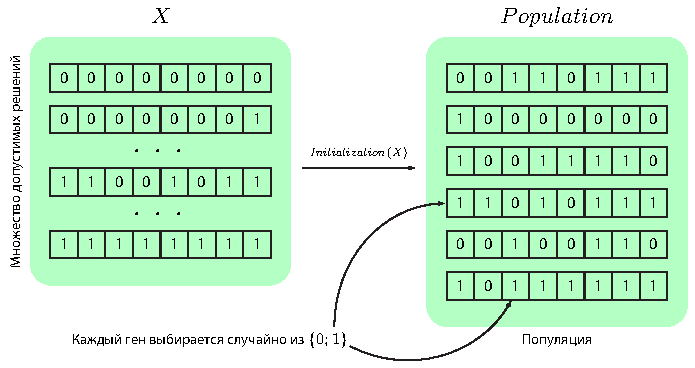
\includegraphics {Initialization.pdf}
  \caption{Инициализация популяции} 
  \label{StandardGA:img:Initialization.pdf}  
\end{figure}


\section{Вычисление функции пригодности} \label{StandardGA:subsection_fit}

Генетический алгоритм не работает с функционалом $ f\left(\bar{x} \right)  $, определяющий эффективность найденных решений. Как видно на схеме (рис. \ref{StandardGA:img:GABinarySheme}), ГА работает с функцией пригодности, которая для каждого индивида из популяции определяется по формуле:

\begin{equation}
\label{StandardGA:eq:fit}
f_{fit}\left( \bar{x}^k\right) = f_1 \left( f_2 \left( f\left( \bar{x}^k\right),g_i\left( \bar{x}^k\right),h_j\left( \bar{x}^k\right)\right),Y \right), 
\end{equation}
\indent где $\bar{x}^k \in Y$, $Y=Population \cup MutChildPopulation$, $k=\overline{1,N}$, $i=\overline{1,m_1}$, $j=\overline{1,m_2}$.

Запишем более кратко для простоты последующих выкладок:

\begin{align}
\label{StandardGA:eq:fitshort}
f_{fit}\left( \bar{x}^k\right) &\equiv f_1^k\left( f_2^k\right) \text{, где }\\
f_2^k&\equiv f_2 \left( f\left( \bar{x}^k\right),g_i\left( \bar{x}^k\right),h_j\left( \bar{x}^k\right)\right), \nonumber\\
f_1^k &\equiv f_1\left(f_2^k \right)\nonumber.
\end{align}

То есть значение функционала $ f\left( \bar{x}^k\right) $ претерпевает два преобразования.

$ f_2^k $ --- преобразование с учетом ограничений, накладываемых на задачу оптимизацию. Например, это может быть штрафы (смертельные, адаптивные и др.). В случае если $ m_1=0 $ и $ m_2=0 $ (задача безусловной оптимизации), то:

\begin{equation}
\label{StandardGA:eq:f_2^k}
f_2^k=f\left( \bar{x}^k\right), k=\overline{1,N}.
\end{equation}

$ f_1^k $ --- преобразование непосредственно по определению функции пригодности. Ее значение требуется в операторе селекции. При использовании пропорциональной селекции выдвигается требование, чтобы показатель эффективности решения был неотрицательной величиной. Функционал $f\left( \bar{x}\right)$ таким свойством не обладает. В литературе не описывается способов приведения к соответствующему виду $f\left( \bar{x}^k\right)$ (или точнее $ f_2^k $). Обычно сразу оговаривается, что $f\left( \bar{x}\right)$ ) обладает необходимыми условиями. Но тестовые функции, на которых проводятся исследования, этими свойствами не обладают. Из-за этого не адекватно сравнивать результаты исследования генетических алгоритмов. Например, при проверке одинаковых модификаций ГА у разных исследователей результаты могут отличаться, так как условия проведения экспериментов разные --- по своей сути решаются разные задачи оптимизации. Поэтому предлагается следующая формула, при использовании которой будет всегда выполняться условие $ f_1^k\geq 0 $:

\begin{equation}
\label{StandardGA:eq:f_1^k}
f_1^k=\left\lbrace \begin{aligned}
\dfrac{f_2^k-I^{min}}{I^{max}-I^{min}},\text { если } I^{max}\neq I^{min}; \\1 ,\text { если } I^{max}= I^{min}.
\end{aligned}\right.
\end{equation}
\begin{equation*}
I^{min}=\min_{\bar{x}^i \in Y} f_2^i, i=\overline{1,N};
\end{equation*}
\begin{equation*}
I^{max}=\max_{\bar{x}^i \in Y} f_2^i, i=\overline{1,N}.
\end{equation*}

\begin{figure} [h] 
  \center
  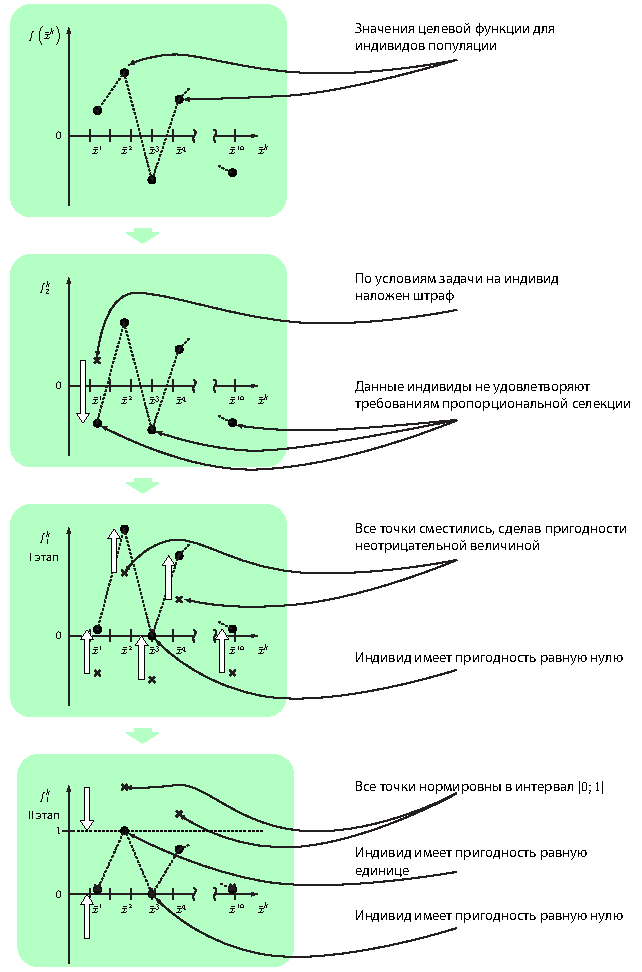
\includegraphics [scale=1] {Fitness}
  \caption{Пример получения пригодности индивидов популяции размера $N=10$} 
  \label{StandardGA:img:Fitness}  
\end{figure}

Отметим, что условие $ f_2^k\geq 0 $ не означает удовлетворения целевой функции требованиям пропорциональной селекции на всем множестве решений, так как условие рассматривает только решения из текущей популяции.

\textbf{Замечание.} Для других типов селекции (ранговая и турнирная) нет требования о неотрицательности функции пригодности. Но монотонное преобразование $ f_1^k $ не изменяет вероятности выбора индивидов из популяции ввиду того, что в данных типах селекции используется только попарное сравнение пригодностей, а не их численных значений.

\textbf{Замечание.} При преобразовании (\ref{StandardGA:eq:f_1^k}) обязательно найдется индивид с вероятностью выбора равной нулю в пропорциональной селекции. То есть в таком случае, всегда хотя бы один индивид в текущем поколении не имеет шансов стать родителем (кроме вырожденного случая, когда все поколение состоит из одного и того же индивида). Существуют другие преобразования $ f_1^k $, лишенные этого недостатка, но они не рассматриваются в данной работе.

\textbf{Замечание.} При использовании пропорциональной селекции  в случае, когда целевая функция (точнее ее преобразование с учетом ограничений) может принимать отрицательные значения, то пригодность одного и того же индивида может изменяться в разных поколениях из-за преобразования (\ref{StandardGA:eq:f_1^k}).

\textbf{Замечание.} Вычисления функции пригодности при программной реализации генетического алгоритма должны проводиться только на этапах «\textbf{Вычисление функции пригодности индивидов}». Во всех остальных операторах, если в формулах используется функция пригодности в виде $f\left( \bar{x}\right) $ или ином виде, то значения функции пригодности должны браться из сохраненных значений, а не расчитываться заново. В противном случае количество вычислений целевой функции не будет совпадать с тем, что задается для запуска генетического алгоритма.

\section{Селекция} \label{StandardGA:subsection_selection}

Селекция --- оператор случайного выбора одного индивида из популяции, основываясь на значениях функции пригодности всех индивидов текущей популяции, для использования его в операторе скрещивания. При этом вероятность выбора у индивидов с более высокой пригодностью выше, чем у индивидов с более низкой пригодностью.

В обычном генетическом алгоритме рассматривается три типа селекции, который определяется параметром $ TypeOfSelection $ из вектора $ DataOfSel $.

\textbf{Пропорциональная селекция.}
\begin{equation}
\label{StandardGA:eq:ProportionalSelection}
TypeOfSelection=ProportionalSelection.
\end{equation}

Вероятность выбора элемента пропорциональна значению пригодности индивида. Данный вид селекции может работать только с неотрицательными значениями пригодности, чем, и вызвано преобразование (\ref{StandardGA:eq:f_1^k}).

Пропорциональная селекция определяется формулой:

\begin{equation}
\label{StandardGA:eq:ProportionalSelection2}
Selection\left( Population, Fitness, DataOfSel\right) = Random\left( \left\lbrace\bar{x}^i | p^i \right\rbrace \right),
\end{equation}
\begin{equation}
p^i=\left\lbrace \begin{aligned}
\dfrac{f_{fit}\left( \bar{x}^i\right) }{\sum_{j=1}^N{f_{fit}\left( \bar{x}^j\right)}},&\text { если }  \exists f_{fit}\left( \bar{x}^k\right)\neq 0 \left( k=\overline{1,N} \right); \\ \dfrac{1}{N} ,&\text { иначе}.
\end{aligned}\right.
\end{equation}

где $ \bar{x}^i \in Population, i=\overline{1,N} $.

Как видим, формула определения вероятности выбора индивида имеет составной вид. Второе условие предназначено для маловероятного случая, когда в популяции все индивиды будут иметь пригодность равную нулю.

$ DataOfSel $ не содержит каких-либо параметров относительно данного типа селекции.

\textbf{Пример.} Пусть $ Fitness=\left\lbrace 0,5; 0,2; 0,1; 0,6; 0,2; 0,4\right\rbrace $. Тогда вероятности выбора индивидов равны:
\begin{flalign*}
p_1&=\frac{0,5}{0,5 + 0,2 + 0,1 + 0,6 + 0,2 + 0,4}=0,25;\\
p_2&=\frac{0,2}{0,5 + 0,2 + 0,1 + 0,6 + 0,2 + 0,4}=0,1;\\
p_3&=\frac{0,1}{0,5 + 0,2 + 0,1 + 0,6 + 0,2 + 0,4}=0,05;\\
p_4&=\frac{0,6}{0,5 + 0,2 + 0,1 + 0,6 + 0,2 + 0,4}=0,3;\\
p_5&=\frac{0,2}{0,5 + 0,2 + 0,1 + 0,6 + 0,2 + 0,4}=0,1;\\
p_6&=\frac{0,4}{0,5 + 0,2 + 0,1 + 0,6 + 0,2 + 0,4}=0,2.
\end{flalign*}

\begin{figure} [h] 
  \center
  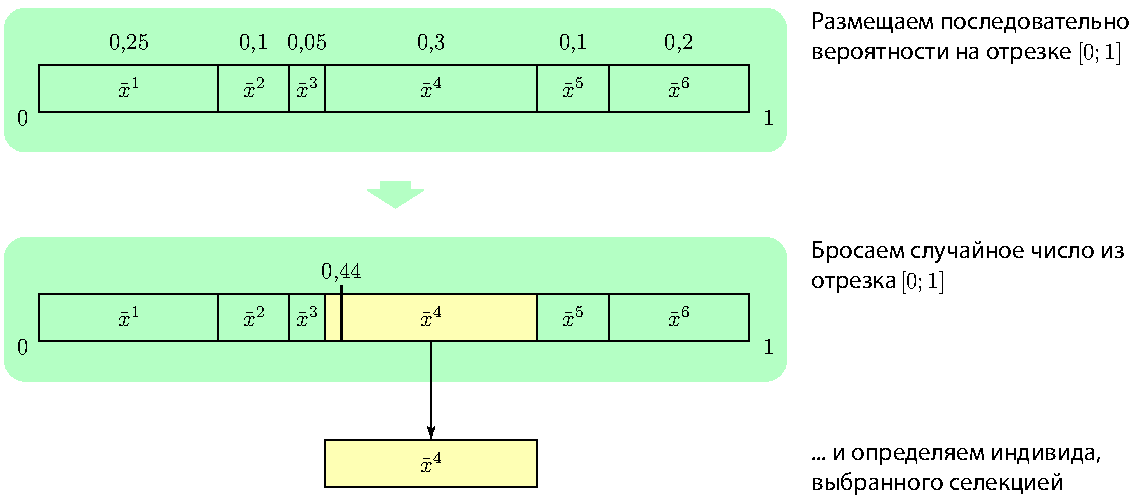
\includegraphics [scale=0.7] {ProportionalSelection}
  \caption{Механизм работы пропорциональной селекции} 
  \label{StandardGA:img:ProportionalSelection}  
\end{figure}

\textbf{Ранговая селекция.}
\begin{equation}
\label{StandardGA:eq:RankSelection}
TypeOfSelection=RankSelection.
\end{equation}

Работает не  с массивом пригодностей напрямую, а массивом нормированных рангов, присваиваемых индивидам на основе значений пригодности. Используется функция, которая проставляет ранги для элементов несортированного массива пригодностей, то есть номера, начиная с $ 1 $, в отсортированном массиве. Если в массиве есть несколько одинаковых элементов, то ранги им присуждаются как среднеарифметические ранги этих элементов в отсортированном массиве. Если это не сделать, то вероятность выбора индивидов одинаковых по функции пригодности будет не равна друг другу, что противоречит идеи оператора селекции. Далее для выбора индивидов используется пропорциональная селекция, работающая с массивом рангов.

Значит, ранговая селекция определяется формулой:

\begin{equation}
\label{StandardGA:eq:RankSelection2}
Selection\left( Population, Fitness, DataOfSel\right) = Random\left( \left\lbrace\bar{x}^i | p^i \right\rbrace \right)
\end{equation}
\begin{equation}
p^i=\dfrac{Rank\left( f_{fit}\left( \bar{x}^i\right)\right)  }{\sum_{j=1}^N{Rank\left( f_{fit}\left( \bar{x}^j\right)\right)}}
\end{equation}
\begin{equation}\label{StandardGA:eq:Rank}
Rank\left( f_{fit}\left( \bar{x}^i\right)\right)=\dfrac{\sum_{j=1}^{N}{NumberOfSorting\left( f_{fit}\left( \bar{x}^i\right), Fitness\right)  \cdot S\left(  f_{fit}\left( \bar{x}^i\right),  f_{fit}\left( \bar{x}^j\right)\right) }}{\sum_{j=1}^{N}{S\left(  f_{fit}\left( \bar{x}^i\right),  f_{fit}\left( \bar{x}^j\right)\right) }}
\end{equation}
\begin{equation}
S\left(  f_{fit}\left( \bar{x}^i\right),  f_{fit}\left( \bar{x}^j\right)\right)= \left\lbrace \begin{array}{l}
1 \text{, если } f_{fit}\left( \bar{x}^i\right)=  f_{fit}\left( \bar{x}^j\right);\\ 0\text{, если } f_{fit}\left( \bar{x}^i\right)\neq  f_{fit}\left( \bar{x}^j\right).
\end{array}\right.
\end{equation}

где $ \bar{x}^i\in Population$, $i=\overline{1,N}.$

$NumberOfSorting\left( f_{fit}\left( \bar{x}^i\right), Fitness\right)$ --- функция, возвращающая номер элемента $ f_{fit}\left( \bar{x}^i\right)) $ в отсортированном массиве $ Fitness $ в порядке возрастания.

Формула (\ref{StandardGA:eq:Rank}) подсчитывает средние арифметические ранги при условии, что в массиве $ Fitness $  могут встречаться одинаковые элементы.

$ DataOfSel $ также не содержит каких-либо параметров относительно данного типа селекции.

\textbf{Пример.} Пусть $ Fitness=\left\lbrace 0,5; 0,2; 0,1; 0,6; 0,2; 0,4\right\rbrace $. Тогда вероятности выбора индивидов равны:
\begin{flalign*}
p_1&=\frac{5}{5+2,5+1+6+2,5+4}=0,238;\\
p_2&=\frac{2,5}{5+2,5+1+6+2,5+4}=0,119;\\
p_3&=\frac{1}{5+2,5+1+6+2,5+4}=0,047;;\\
p_4&=\frac{6}{5+2,5+1+6+2,5+4}=0,286;\\
p_5&=\frac{2,5}{5+2,5+1+6+2,5+4}=0,119;\\
p_6&=\frac{4}{5+2,5+1+6+2,5+4}=0,190.
\end{flalign*}

\begin{figure} [h] 
  \center
  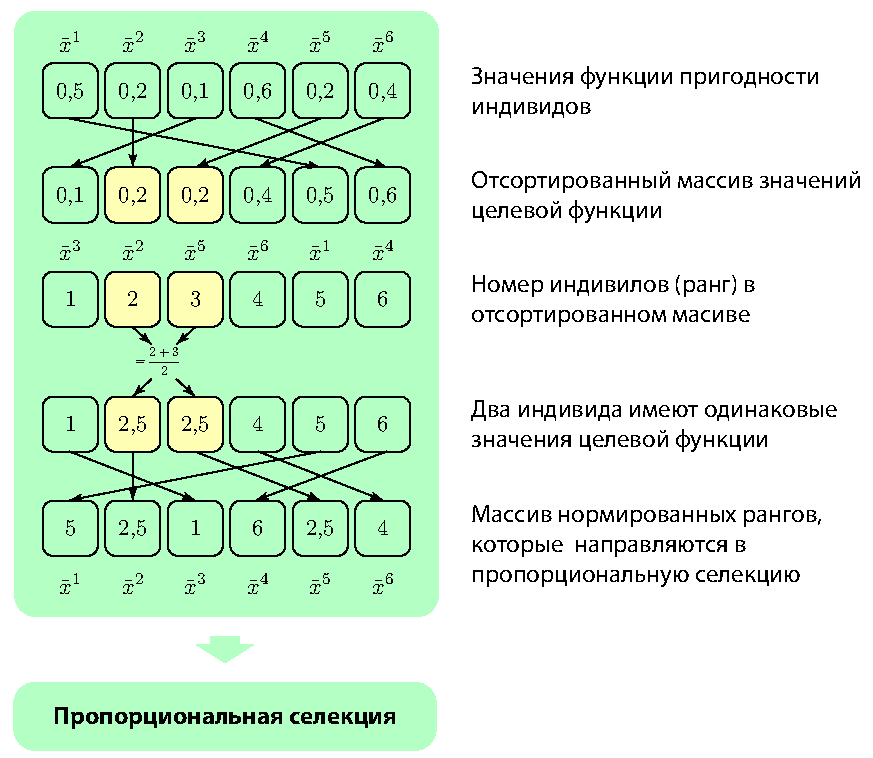
\includegraphics [scale=0.8] {RankSelection}
  \caption{Механизм работы ранговой селекции} 
  \label{StandardGA:img:RankSelection}  
\end{figure}

\textbf{Турнирная селекция.}
\begin{equation}
\label{StandardGA:eq:TournamentSelection}
TypeOfSelection=TournamentSelection.
\end{equation}

Из популяции с равной вероятностью выбираются индивиды в количестве $ T $ (размер турнира), где $ 2\leq T\leq N $. При этом каждый индивид может попасть в группу (турнир) только один раз (турнирная селекция без возвращения). Из данной группы выбирается индивид с наибольшей пригодностью.

Значит, турнирная селекция определяется формулой:
\begin{align}
\label{StandardGA:eq:TournamentSelection2}
Selection\left( Population, Fitness, DataOfSel\right) = \arg{\max_{\bar{x}\in H} {f_{fit}\left( \bar{x}\right) }}, \text{где }\\
H=\left\lbrace h^i | h_i=Random \left( Population/\left( \left\lbrace h^1\right\rbrace \cup \left\lbrace h^2\right\rbrace \cup \ldots  \cup \left\lbrace h^{i-1}\right\rbrace\right) \right) \right\rbrace, i=\overline{1,T}\nonumber.
\end{align}

Турнирная селекция является единственным типом данного оператора, который добавляет в $ DataOfSel $ дополнительный параметр – размер турнира $ T $. Обычно выбирают значение этого параметра равное $ T=2 $.

\textbf{Пример.} Массив возьмем тот же, что и в предыдущих примерах $ Fitness=\left\lbrace 0,5; 0,2; 0,1; 0,6; 0,2; 0,4\right\rbrace $. Размер турнира равен $ T=3 $. Пример работы оператора показан на рисунке:

\begin{figure} [h] 
  \center
  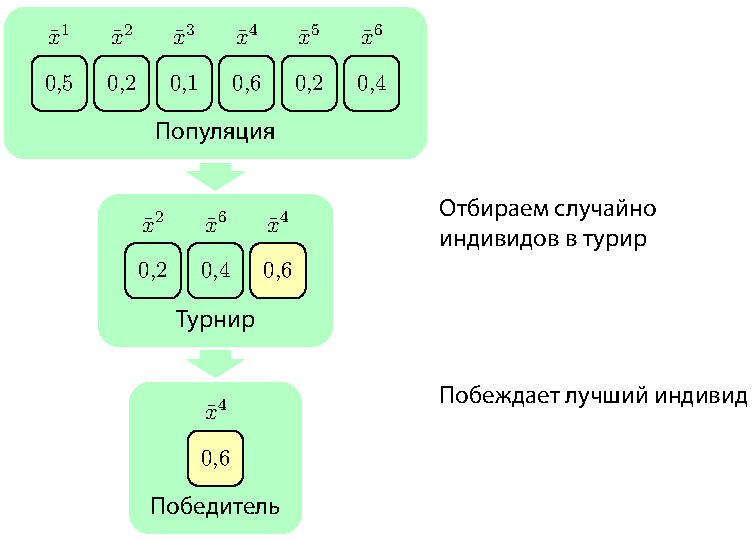
\includegraphics [scale=0.8] {TournamentSelection}
  \caption{Механизм работы турнирной селекции} 
  \label{StandardGA:img:TournamentSelection}  
\end{figure}

Итак, мы рассмотрели используемые варианты селекции. Тогда можно составить вектор параметров оператора селекции $ DataOfSel $:

\begin{equation}
\label{StandardGA:eq:DataOfSel}
DataOfSel=\left( \begin{array}{c} TypeOfSel \\ T \end{array} \right).
\end{equation}

\textbf{Замечание.} Часто в литературе наряду с рассмотренными ниже тремя видами селекции упоминается элитарная селекция (элитная селекция, селекция элитизма). Этот оператор не является селекцией по определению этого оператора. В стандарте включен в состав одного из вида оператора формирования нового поколения из родителей и потомков.

\textbf{Замечание.} Часто при программировании турнирной селекции реализуется такой вариант, при котором один и тот же индивид из популяции может быть выбран в турнир несколько раз. Это происходит из-за простоты программирования данного способа, но является недопустимым при реализации вышеупомянутой селекции. В противном случае мы получаем модифицированный вариант турнирной селекции с возвращением, который требует дополнительных исследований.

Разумеется, выбранный индивид для участия в турнире, может принять участие в других турнирах.

\textbf{Замечание.} Часто в литературе встречаются различные варианты ранговой селекции, связанные с преобразованием значений рангов (возведение в квадрат и др.) В данной работе эти варианты не рассматриваются.

\textbf{Замечание.} Программировать оператор селекции рекомендуется таким образом, чтобы он возвращал не индивида, а его номер в популяции.

\textbf{Замечание.} Если при выполнении селекции сравниваются два разных индивида с одинаковыми значениями функций пригодности, то выбирается первый из них.

\section{Скрещивание} \label{StandardGA:subsection_Crossover}

\textbf{Скрещивание (кроссовер)} --- оператор случайного формирования нового индивида из двух выбранных родителей с сохранением признаков обоих родителей.

В обычном генетическом алгоритме рассматривается три типа скрещивания, который определяется параметром $ TypeOfCrossover $ из вектора $ DataOfCros $.

\textbf{Одноточечное скрещивание.}
\begin{equation}
\label{StandardGA:eq:SinglepointCrossover}
TypeOfCrossover=SinglepointCrossover.
\end{equation}

Пусть имеется два родителя (родительские хромосомы) $ \overline{Parent}^1 $ и $ \overline{Parent}^2$. В случайном месте происходит разрыв между двумя позициями генов в обеих хромосомах. После этого хромосомы обмениваются частями, в результате чего образуются два потомка. Из них выбирается случайно один потомок, который и передается в качестве результата оператора скрещивания. То есть скрещивание происходит по формулам:

\begin{align}
\label{StandardGA:eq:SinglepointCrossover2}
&Crossover \left( \overline{Parent}^1, \overline{Parent}^2, DataOfCros\right)=Random \left(\left\lbrace \overline{Offspring}^1; \overline{Offspring}^2\right\rbrace  \right), \\
&R=Random\left( \left\lbrace 2; 3; \ldots; n\right\rbrace \right); \nonumber \\
& \overline{Offspring}^1_i=\overline{Parent}^1_i, i=\overline{1,R-1};\nonumber\\
&  \overline{Offspring}^1_i=\overline{Parent}^2_i, i=\overline{R,n};\nonumber\\
&\overline{Offspring}^2_i=\overline{Parent}^2_i, i=\overline{1,R-1};\nonumber\\
& \overline{Offspring}^2_i=\overline{Parent}^1_i, i=\overline{R,n};\nonumber\\
&\overline{Offspring}^1\in X, \overline{Offspring}^2\in X.\nonumber
\end{align}

$ DataOfCros $ не содержит каких-либо параметров относительно данного типа скрещивания.

\textbf{Пример.} Для всех видов скрещивания будем использовать двух родителей: $\overline{Parent}^1\hm={\left( 0; 1; 0; 1; 1; 1; 0; 0\right)}^\mathrm{T}  $ и $\overline{Parent}^2={\left( 1; 1; 0; 0; 1; 0; 1\right)}^\mathrm{T}  $. Одноточечное скрещивание показано на рисунке:

\begin{figure} [h] 
  \center
  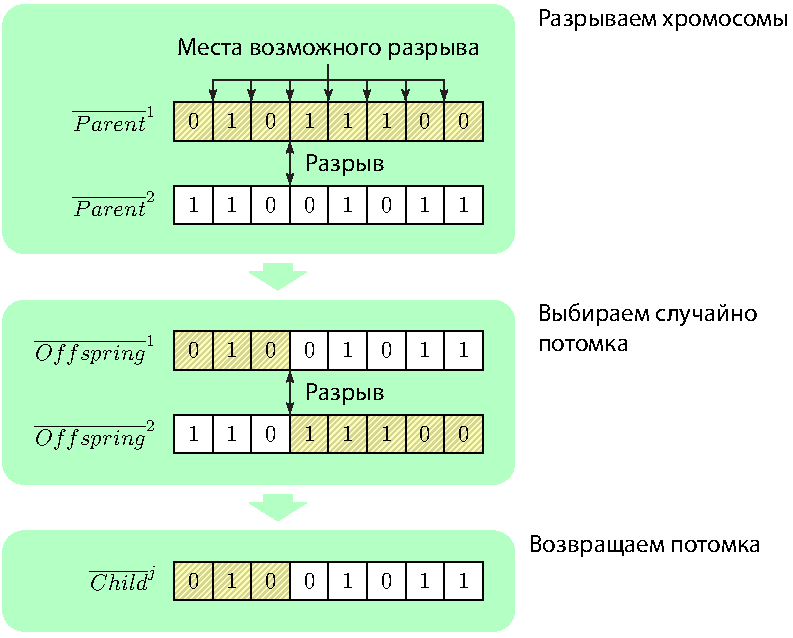
\includegraphics [scale=0.8] {SinglepointCrossover}
  \caption{Механизм работы одноточечного скрещивания} 
  \label{StandardGA:img:SinglepointCrossover}  
\end{figure}

\textbf{Двухточечное скрещивание.}
\begin{equation}
\label{StandardGA:eq:TwopointCrossover}
TypeOfCrossover=TwopointCrossover.
\end{equation}

Пусть имеется два родителя (родительские хромосомы) $\overline{Parent}^1$ и $\overline{Parent}^2$. В двух случайных местах происходят разрывы между двумя позициями генов в обеих хромосомах. После этого хромосомы обмениваются частями, в результате чего образуются два потомка. Из них выбирается случайно один потомок, который и передается в качестве результата оператора скрещивания. То есть скрещивание происходит по формулам:

\begin{align}
\label{StandardGA:eq:TwopointCrossover2}
&Crossover \left( \overline{Parent}^1, \overline{Parent}^2, DataOfCros\right)=Random \left(\left\lbrace \overline{Offspring}^1; \overline{Offspring}^2\right\rbrace  \right), \\
&r_1=Random\left( \left\lbrace 2; 3; \ldots; n\right\rbrace \right); \nonumber \\
&r_2=Random\left( \left\lbrace 2; 3; \ldots; n\right\rbrace \right); \nonumber \\
&R_1=\min \left( r_1, r_2\right) ; \nonumber \\
&R_2=\max \left( r_1, r_2\right) ; \nonumber \\
& \overline{Offspring}^1_i=\overline{Parent}^1_i, i=\overline{1,R_1-1};\nonumber\\
& \overline{Offspring}^1_i=\overline{Parent}^2_i, i=\overline{R_1,R_2-1};\nonumber\\
&  \overline{Offspring}^1_i=\overline{Parent}^1_i, i=\overline{R_2,n};\nonumber\\
& \overline{Offspring}^2_i=\overline{Parent}^2_i, i=\overline{1,R_1-1};\nonumber\\
& \overline{Offspring}^2_i=\overline{Parent}^1_i, i=\overline{R_1,R_2-1};\nonumber\\
&  \overline{Offspring}^2_i=\overline{Parent}^2_i, i=\overline{R_2,n};\nonumber\\
&\overline{Offspring}^1\in X, \overline{Offspring}^2\in X.\nonumber
\end{align}

$ DataOfCros $ не содержит каких-либо параметров относительно данного типа скрещивания.

\textbf{Пример.} Двухточечное скрещивание показано на рисунке:

\begin{figure} [h]
  \center
  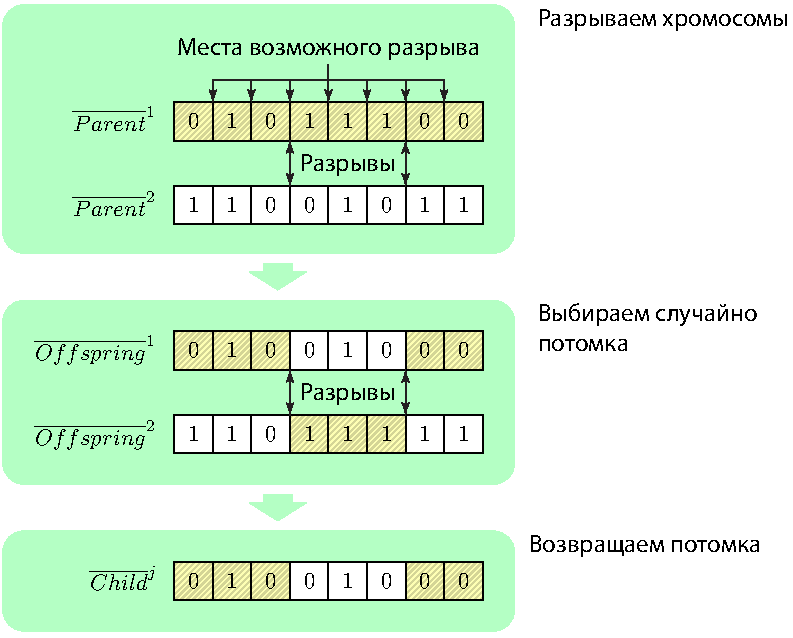
\includegraphics [scale=0.8] {TwopointCrossover}
  \caption{Механизм работы двухточечного скрещивания} 
  \label{StandardGA:img:TwopointCrossover}  
\end{figure}

\textbf{Равномерное скрещивание.}
\begin{equation}
\label{StandardGA:eq:UniformCrossover}
TypeOfCrossover=UniformCrossover.
\end{equation}

Пусть имеется два родителя (родительские хромосомы) $\overline{Parent}^1$ и $\overline{Parent}^2$. Потомок состоит из генов, каждый из которых выбран случайно из генов родителей на соответствующих позициях. То есть скрещивание происходит по формулам:

\begin{align}
\label{StandardGA:eq:UniformCrossover2}
&Crossover \left( \overline{Parent}^1, \overline{Parent}^2, DataOfCros\right) = \overline{Offspring};\\
& \overline{Offspring}_i=Random\left( \left\lbrace \overline{Parent}^1_i;\overline{Parent}^2_i\right\rbrace \right), i=\overline{1,n} ;\nonumber\\
&\overline{Offspring}\in X.\nonumber
\end{align}

$ DataOfCros $ не содержит каких-либо параметров относительно данного типа скрещивания.

\textbf{Пример.} Равномерное скрещивание показано на рисунке:

\begin{figure} [h]
  \center
  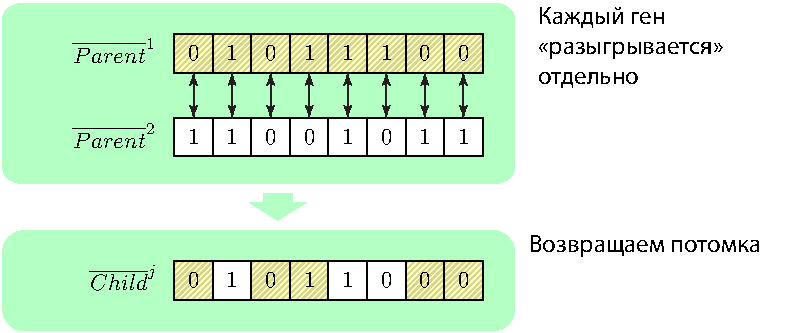
\includegraphics [scale=0.7] {UniformCrossover}
  \caption{Механизм работы равномерного скрещивания} 
  \label{StandardGA:img:UniformCrossover}  
\end{figure}

Итак, мы рассмотрели используемые варианты скрещивания. Тогда можно составить вектор параметров оператора скрещивания $ DataOfCros $:

\textbf{Равномерное скрещивание.}
\begin{equation}
\label{StandardGA:eq:DataOfCros}
DataOfCros=\left( TypeOfCros\right) .
\end{equation}

\textbf{Замечание.} В одноточечном и двухточечном скрещивании разрыв хромосомы может произойти только между двумя генами, то есть в начале или конце хромосомы разрыв произойти не может, что является частой ошибкой при программировании. Такая операция не даст новых решений.

\textbf{Замечание.} В литературе присутствует два подхода к оператору скрещивания. Согласно первому в результате скрещивания получаются два потомка, которые оба попадают в популяцию потомков. Но этот способ накладывает ограничение на размер популяции $ N $: он должен быть четным. В данной работе используется второй подход, согласно которому в популяцию потомков попадает только один потомок, отобранный случайно. Есть варианты  в литературе, когда отбирается потомок с наилучшей пригодностью, но это в два раза увеличивает число вычислений функции, причем половина из них идет на вычисление функции пригодности индивидов, которые не примут участие в существовании популяции.

\textbf{Замечание.} В качестве двух родителей может выбраться один и тот же индивид $ \overline{Parent}^1\hm= \overline{Parent}^2 $. Это не запрещается в отличие от запрета попадания одного и того же индивида в турнир в турнирной селекции.

\textbf{Замечание.} В литературе в качестве одного из параметров скрещивания выступает вероятность скрещивания. Но часто она принимается за единицу, а многими исследователями вовсе опускается. В Стандарте (здесь описывается простейший вариант генетического алгоритма) данный параметр опущен.

Вероятность скрещивания меньше $ 1 $ исполняет роль операции клонирования. Хотя в Стандарте мы ее опустили, клонирование выполняется за счет селекции с повторением, то есть возможна реализация скрещивания одинаковых решений (см. предыдущее замечание)  --- аналог клонирования с очень низкой вероятностью.

\textbf{Замечание.} В двухточечном скрещивании точки разрыва могут совпасть. Тогда потомок будет совпадать с одним из родителей.

\textbf{Замечание.} Обратите внимание, что при описании оператора скрещивания для обозначения потомков используются $ \overline{Offspring} $, в схеме работы стандартного генетического алгоритма на бинарных строках $ \overline{Child} $. Это объясняется следующим образом. $ \overline{Child} $ используется для обозначения итогового потомка, который является результатом оператора скрещивания, тогда как $ \overline{Offspring} $ служит для обозначения временного потомка внутри работы оператора, и временных потомков может получиться несколько. Один из них, который выбирается, как описано выше, и становится возвращаемым $ \overline{Child} $.

\section{Мутация} \label{StandardGA:subsection_Mutation}

\textbf{Мутация} --- оператор случайного изменения всех потомков из популяции. Цель данного оператора  не получить более лучшее решение, а разнообразить многообразие рассматриваемых индивидов. Обычно мутация предполагает незначительное изменение потомков. При выполнении оператора каждый ген каждого индивида с некоторой заданной вероятностью  $ ProbabilityOfMutation $ мутирует, то есть меняет свое значение на противоположное. Мутация происходит по формулам:
\begin{align}
\label{StandardGA:eq:Mutation}
&\overline{MutChild}_j^i=\left\lbrace \begin{aligned}
\overline{Child}_j^i&\text{, если } random \left(0, 1 \right)>ProbabilityOfMutation; \\
1-\overline{Child}_j^i&\text{, иначе }.
\end{aligned}\right.\\
&\overline{Child}^i \in ChildPopulation, i=\overline{1,N},\nonumber\\
&\overline{MutChild}^i \in X, i=\overline{1,N}.\nonumber
\end{align}

Обычно в генетическом алгоритме вероятность мутации выбирается из трех вариантов: слабая ($ Weak $), средняя ($ Average $) и сильная ($ Strong $) мутация.
Отсюда вероятность мутации определяется формулой:
\begin{align}
\label{StandardGA:eq:ProbabilityOfMutation}
ProbabilityOfMutation\left( TypeOfMutation\right) =\\ =\left\lbrace \begin{aligned}
\frac{1}{3n}&\text{, если }TypeOfMutation=Weak; \\ \frac{1}{n}&\text{, если }TypeOfMutation=Average; \\ min\left(1, \frac{3}{n}\right) &\text{, если }TypeOfMutation=Strong.
\end{aligned}\right.\nonumber
\end{align}

Здесь
\begin{equation}
\label{StandardGA:eq:TypeOfMutation}
TypeOfMutation \in \left\lbrace Weak; Average;Strong\right\rbrace ,
\end{equation}

$ n $ --- длина вектора $ \bar{x}\in X $ бинарной задачи оптимизации.

Составим вектор параметров оператора мутации $ DataOfMut $:
\begin{equation}
\label{StandardGA:eq:DataOfMut}
DataOfMut=\left( TypeOfMutation\right) .
\end{equation}

\textbf{Замечание.} Определение сильной мутации через $ min\left(1, \frac{3}{n}\right) $  связано с тем, что при  $ n<3 $ вероятность мутации становится больше $ 1 $, что недопустимо. Но при программировании это не вызывает отклонений в работе генетического алгоритма, к тому же использование ГА для столь малых размерностей нецелесообразно.

\textbf{Замечание.} Часто в литературе под мутацией понимается не оператор над всеми потомками, а оператор над каждым в отдельности. Никакой принципиальной разницы в двух этих подходах нет.

\textbf{Пример.} На риc. \ref{StandardGA:img:Mutation} показана мутация одного из индивидов из популяции.

\begin{figure} [h]
  \center
  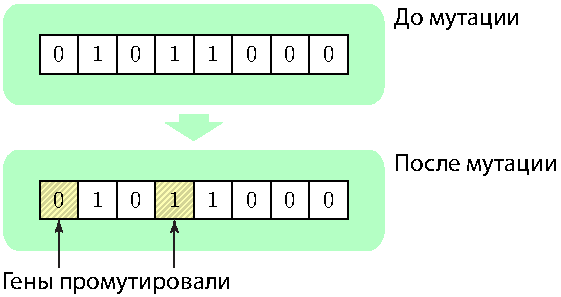
\includegraphics [scale=0.7] {Mutation}
  \caption{Механизм работы мутации} 
  \label{StandardGA:img:Mutation}  
\end{figure}

\section{Формирование нового поколения} \label{StandardGA:subsection_GenerationForming}

\textbf{Формирование нового поколения} --- оператор формирования нового поколения из массива родителей и получившихся потомков с использованием уже известных значений функции пригодности, как родителей, так и потомков.

В обычном генетическом алгоритме используется два типа формирования нового поколения, который определяется параметром $ TypeOfGenerationForming $ из вектора $ DataOfForm $.

\textbf{Только потомки.}
\begin{equation}
\label{StandardGA:eq:OnlyOffspringGenerationForming}
TypeOfGenerationForming=OnlyOffspringGenerationForming.
\end{equation}

Данная схема предполагает формирование нового поколения из потомков и родителей таким, что в новое поколение попадают только потомки. Данный тип формирования нового поколения определяется формулой:
\begin{equation}
\label{StandardGA:eq:OnlyOffspringGenerationForming2}
Forming \left( \begin{array}{c} Population\\MutChildPopulation\\Fitness\\FitnessOfMutChild\\DataOfForm\end{array}\right) =\left( \begin{array}{c} MutChildPopulation\\FitnessOfMutChild\end{array}\right).
\end{equation}

$ DataOfForm $ не содержит каких-либо параметров относительно данного типа формирования нового поколения.

\textbf{Только потомки и копия лучшего индивида.}
\begin{equation}
\label{StandardGA:eq:OnlyOffspringWithBestGenerationForming}
TypeOfGenerationForming=OnlyOffspringWithBestGenerationForming.
\end{equation}

Данная схема предполагает формирование нового поколения из потомков и родителей таким, что в новое поколение попадают только потомки (без одного) и копия лучшего индивида $ \overline{Best} $ (лучшего за всё время работы генетического алгоритма, а не только текущего поколения). В русской литературе данный способ часто называют селекцией элитизма. Данный тип формирования нового поколения определяется формулой:

\begin{align}
\label{StandardGA:eq:OnlyOffspringWithBestGenerationForming2}
&Forming \left( \begin{array}{c} Population\\MutChildPopulation\\Fitness\\FitnessOfMutChild\\DataOfForm\end{array}\right) =\left( \begin{array}{c} \left\lbrace \bar{x}^i\right\rbrace \\\left\lbrace f^i\right\rbrace\end{array}\right),\\&\bar{x}^i=\left\lbrace \begin{aligned}
\overline{Best}&\text{, если }i=0; \\ \overline{MutChild}^i&\text{, если }i\neq 0;
\end{aligned}\right.\nonumber\\
&f_i=f\left( \bar{x}_i\right), i=\overline{1,N}.\nonumber
\end{align}

$ DataOfForm $ не содержит каких-либо параметров относительно данного типа формирования нового поколения.

Итак, мы рассмотрели используемые варианты формирования нового поколения. Составим вектор параметров оператора формирования нового поколения:
\begin{equation}
\label{StandardGA:eq:DataOfForm}
DataOfForm=\left( TypeOfForm\right) .
\end{equation}

\clearpage